\KOMAoptions{paper=A4}
\recalctypearea
{\scriptsize
\section{Array Leeway (2-D Arrays)}
\begin{topics}
2-D arrays, function \& arrays and previous sections.
\end{topics}
\subsection{Case Converter}
\textbf{Problem Statement:}\\
Convert a given text into different cases as mentioned below
\begin{description}
	\item[aLtErNaTiNg CaPs] Start with a lower case letter and then keep switching between upper case and lower case letters alternatingly.
	\item[Capitalize Word] Capitalize the first letter of each word and convert all other letters of that word to lower case.
	\item[lower case] Convert every alphabet to lower case.
	\item[Sentence case] Capitalize the first letter of each sentence and convert all other letters of that sentence to lower case. A sentence only ends with a full stop (`.') .
	\item[tOGGLE cASE] Uncapitalize the first letter of each word and convert all other letters of that word to upper case.
	\item[UPPER CASE] Convert every alphabet to upper case.
\end{description}
\begin{note}
	In all above cases, ignore non-alphabetic characters.
\end{note}
\begin{testcases}
	{sentence\_length\quad x \hfill(x is either a/c/l/s/t/u denoting the case to convert to or e for all cases)\\
	sentence\hfill(entire sentence in a line, the sentence\_length includes spaces)}
	{The sentence converted into x case\hfill{(already taken care of in \href{https://github.com/paramrathour/CS-101/tree/main/Starter Codes/Case Converter.cpp}{Starter Code})}}
	{$1 \leq \text{sentence\_length} \leq 10000$}
	{479\quad e\\The Earth is a very small stage in a vast cosmic arena. Think of the endless cruelties visited by the inhabitants of one corner of this pixel on the scarcely distinguishable inhabitants of some other corner, how frequent their misunderstandings, how eager they are to kill one another, how fervent their hatreds. Think of the rivers of blood spilled by all those generals and emperors so that, in glory and triumph, they could become the momentary masters of a fraction of a dot.}
	{tHe EaRtH iS a VeRy SmAlL sTaGe In A vAsT cOsMiC aReNa. ThInK oF tHe EnDlEsS cRuElTiEs ViSiTeD bY tHe InHaBiTaNtS oF oNe CoRnEr Of ThIs PiXeL oN tHe ScArCeLy DiStInGuIsHaBlE iNhAbItAnTs Of SoMe OtHeR cOrNeR, hOw FrEqUeNt ThEiR mIsUnDeRsTaNdInGs, HoW eAgEr ThEy ArE tO kIlL oNe AnOtHeR, hOw FeRvEnT tHeIr HaTrEdS. tHiNk Of ThE rIvErS oF bLoOd SpIlLeD bY aLl ThOsE gEnErAlS aNd EmPeRoRs So ThAt, In GlOrY aNd TrIuMpH, tHeY cOuLd BeCoMe ThE mOmEnTaRy MaStErS oF a FrAcTiOn Of A dOt.\\\\
The Earth Is A Very Small Stage In A Vast Cosmic Arena. Think Of The Endless Cruelties Visited By The Inhabitants Of One Corner Of This Pixel On The Scarcely Distinguishable Inhabitants Of Some Other Corner, How Frequent Their Misunderstandings, How Eager They Are To Kill One Another, How Fervent Their Hatreds. Think Of The Rivers Of Blood Spilled By All Those Generals And Emperors So That, In Glory And Triumph, They Could Become The Momentary Masters Of A Fraction Of A Dot.\\\\
the earth is a very small stage in a vast cosmic arena. think of the endless cruelties visited by the inhabitants of one corner of this pixel on the scarcely distinguishable inhabitants of some other corner, how frequent their misunderstandings, how eager they are to kill one another, how fervent their hatreds. think of the rivers of blood spilled by all those generals and emperors so that, in glory and triumph, they could become the momentary masters of a fraction of a dot.\\\\
The earth is a very small stage in a vast cosmic arena. Think of the endless cruelties visited by the inhabitants of one corner of this pixel on the scarcely distinguishable inhabitants of some other corner, how frequent their misunderstandings, how eager they are to kill one another, how fervent their hatreds. Think of the rivers of blood spilled by all those generals and emperors so that, in glory and triumph, they could become the momentary masters of a fraction of a dot.\\\\
tHE eARTH iS a vERY sMALL sTAGE iN a vAST cOSMIC aRENA. tHINK oF tHE eNDLESS cRUELTIES vISITED bY tHE iNHABITANTS oF oNE cORNER oF tHIS pIXEL oN tHE sCARCELY dISTINGUISHABLE iNHABITANTS oF sOME oTHER cORNER, hOW fREQUENT tHEIR mISUNDERSTANDINGS, hOW eAGER tHEY aRE tO kILL oNE aNOTHER, hOW fERVENT tHEIR hATREDS. tHINK oF tHE rIVERS oF bLOOD sPILLED bY aLL tHOSE gENERALS aND eMPERORS sO tHAT, iN gLORY aND tRIUMPH, tHEY cOULD bECOME tHE mOMENTARY mASTERS oF a fRACTION oF a dOT.\\\\
THE EARTH IS A VERY SMALL STAGE IN A VAST COSMIC ARENA. THINK OF THE ENDLESS CRUELTIES VISITED BY THE INHABITANTS OF ONE CORNER OF THIS PIXEL ON THE SCARCELY DISTINGUISHABLE INHABITANTS OF SOME OTHER CORNER, HOW FREQUENT THEIR MISUNDERSTANDINGS, HOW EAGER THEY ARE TO KILL ONE ANOTHER, HOW FERVENT THEIR HATREDS. THINK OF THE RIVERS OF BLOOD SPILLED BY ALL THOSE GENERALS AND EMPERORS SO THAT, IN GLORY AND TRIUMPH, THEY COULD BECOME THE MOMENTARY MASTERS OF A FRACTION OF A DOT.}
	{https://github.com/paramrathour/CS-101/tree/main/Starter Codes/Case Converter.cpp}
\end{testcases}
}
\KOMAoptions{paper=A4}
\recalctypearea
\subsection{Spiral Grid}
\textbf{Problem Statement:}\\
Generate a grid containing numbers from $1$ to $n^2$ such that $1$ is at center and then the numbers spiral outwards from $1$ in counterclockwise direction. Also, make sure each element of grid is equally spaced as shown in \ref{fig:spiralgrid}.
\begin{note}
	If $n$ is even then choose the left-bottom element from the four possible centers.
\end{note}
\begin{comment}
	\begin{figure}[H]
		\centering
		\begin{subfigure}{0.4\linewidth}
			\centering
			\begin{tabular}{rrrr}
			16 & 15 & 14 & 13 \\
			5  & 4  & 3  & 12 \\
			6  & 1  & 2  & 11 \\
			7  & 8  & 9  & 10
			\end{tabular}
			\caption{$n=4$}
		\end{subfigure}
		\begin{subfigure}{0.4\linewidth}
			\centering
			\begin{tabular}{rrrrr}
			17 & 16 & 15 & 14 & 13 \\
			18 & 5  & 4  & 3  & 12 \\
			19 & 6  & 1  & 2  & 11 \\
			20 & 7  & 8  & 9  & 10 \\
			21 & 22 & 23 & 24 & 25
			\end{tabular}
			\caption{$n=5$}
		\end{subfigure}
		\caption{Spiral Grid}
		\label{fig:spiralgrid}
	\end{figure}
\end{comment}
\begin{testcasesMore}
	{$t$ \hfill(number of test cases, an integer)\\$n_1\ n_2\ \ldots\ n_t$ \hfill($t$ space seperated integers for each testcase)}
	{Required spiral grid of $n_i^2$ numbers with appropriate spacing}
	{$1 \leq n_i \leq 100$}
	{5\\1 2 3 6 15}
	{\vspace{-2em}\begin{figure}[H]
		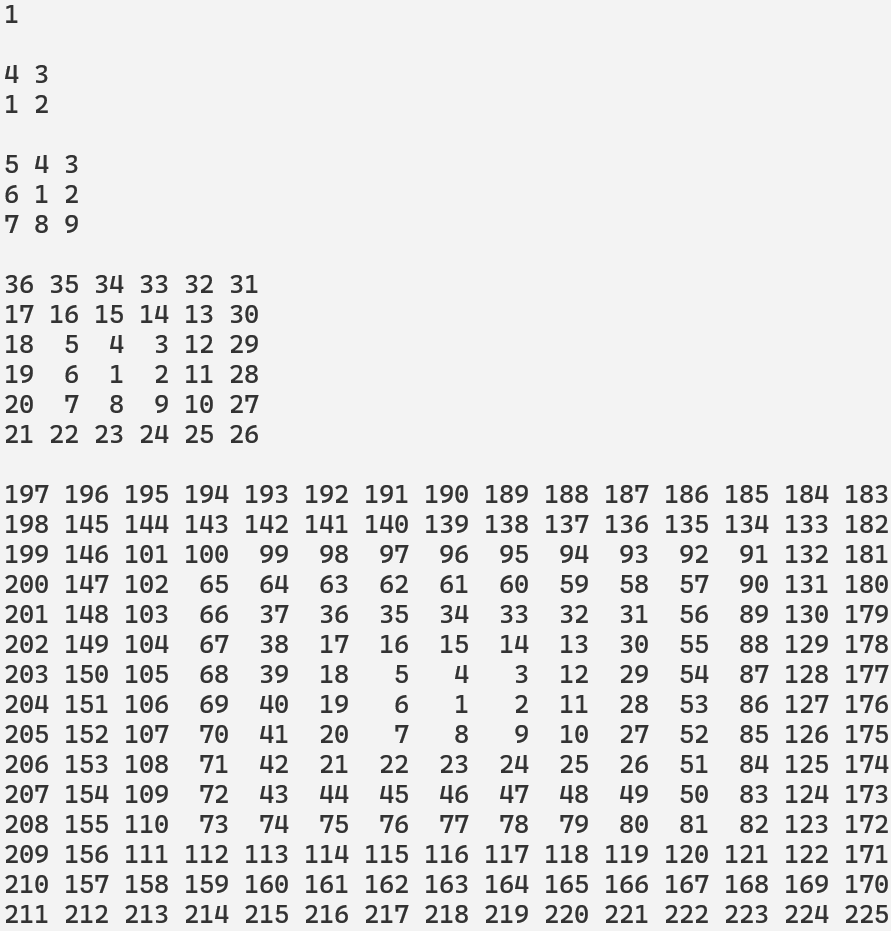
\includegraphics[width=0.5\linewidth]{Spiral Grid.png}
		\caption{Sample Output}
		\label{fig:spiralgrid}
	\end{figure}
	}
	{https://github.com/paramrathour/CS-101/tree/main/Test Cases/Spiral Grid/Input.txt}
	{https://github.com/paramrathour/CS-101/tree/main/Test Cases/Spiral Grid/Output.txt}
	{https://github.com/paramrathour/CS-101/tree/main/Starter Codes/Spiral Grid.cpp}
\end{testcasesMore}
\subsection{Minesweeper}
In the game of Minesweeper, there is an $m\times n$ board which has exactly $k$ mines hidden. The aim is to ``clear'' the board by clicking on cells with no mine and avoiding clicking on any mine. By clicking on a cell with no mine, the player gets the number of neighbouring mines of that cell by the below rule
\begin{itemize}	
	\item If the cell $c$ is not at the boundary (\ref{fig:minecnb}) then it is the number of mines in a $3\times3$ square with that centre $c$.
	\item If the cell $c$ is at the boundary (\ref{fig:minecb1}, \ref{fig:minecb1}) even then $c$ cell is considered as the centre of $3\times3$ square; but, only some of the cells of the constructed square will lie inside the board.
\end{itemize}
\begin{figure}[H]
	\centering
	\begin{subfigure}[t]{0.25\linewidth}
		\centering
		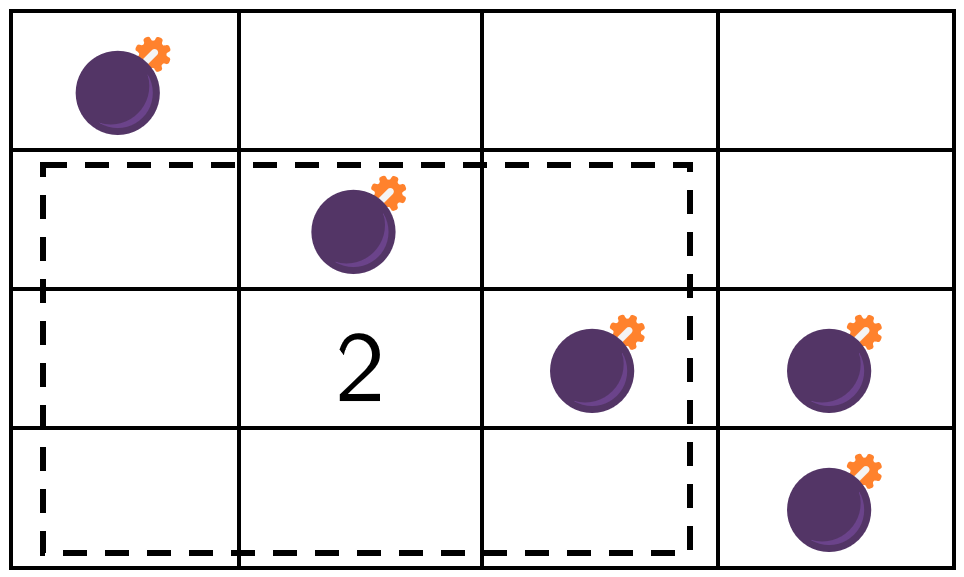
\includegraphics[height = 0.528\textwidth]{Minesweeper/middle.png}
		\caption{Cell is not at the boundary}
		\label{fig:minecnb}
	\end{subfigure}
	\begin{subfigure}[t]{0.22\linewidth}
		\centering
		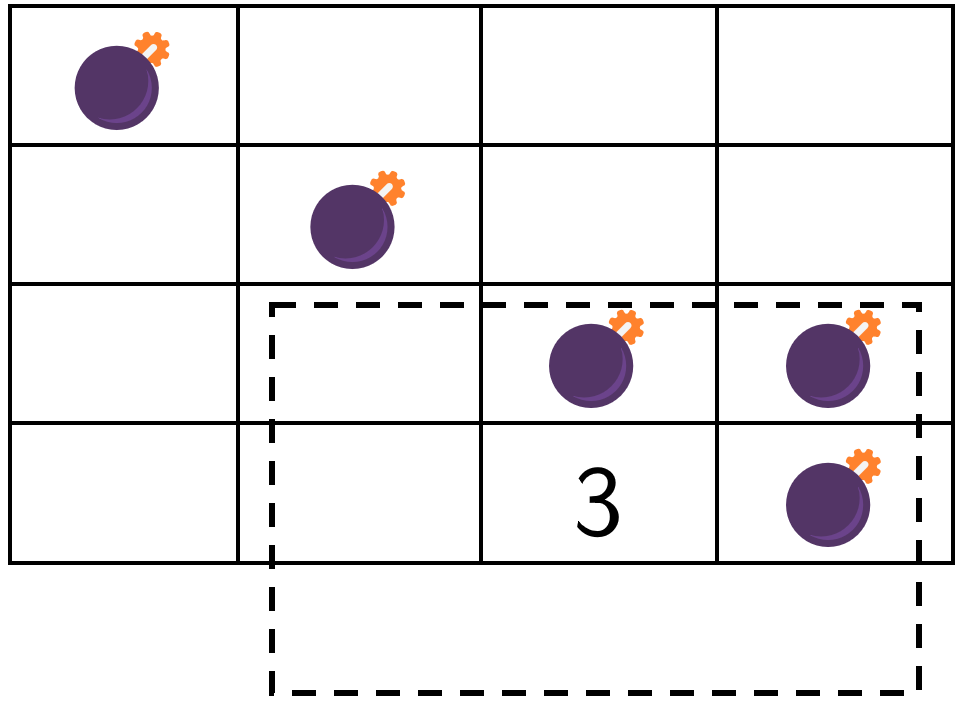
\includegraphics[height = 0.6\textwidth]{Minesweeper/bottom.png}
		\caption{Cell is at the boundary}
		\label{fig:minecb1}
	\end{subfigure}
	\begin{subfigure}[t]{0.22\linewidth}
		\centering
		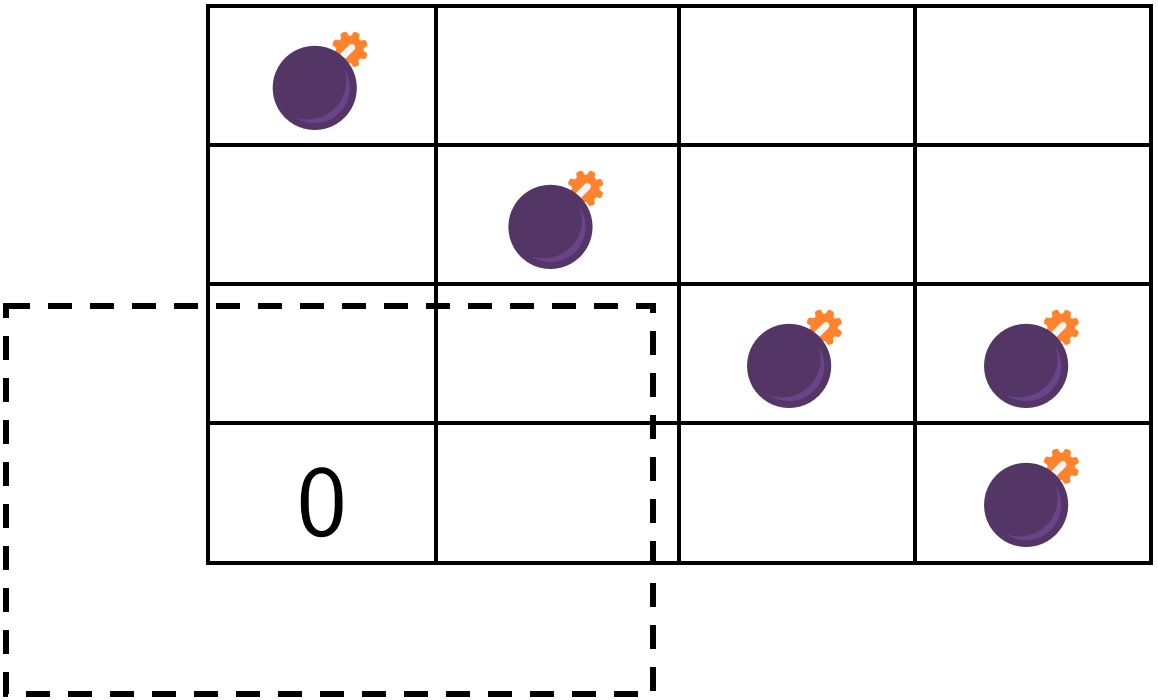
\includegraphics[height = 0.6\textwidth]{Minesweeper/corner.png}
		\caption{Cell is at the boundary}
		\label{fig:minecb2}
	\end{subfigure}
	\begin{subfigure}[t]{0.22\linewidth}
		\centering
		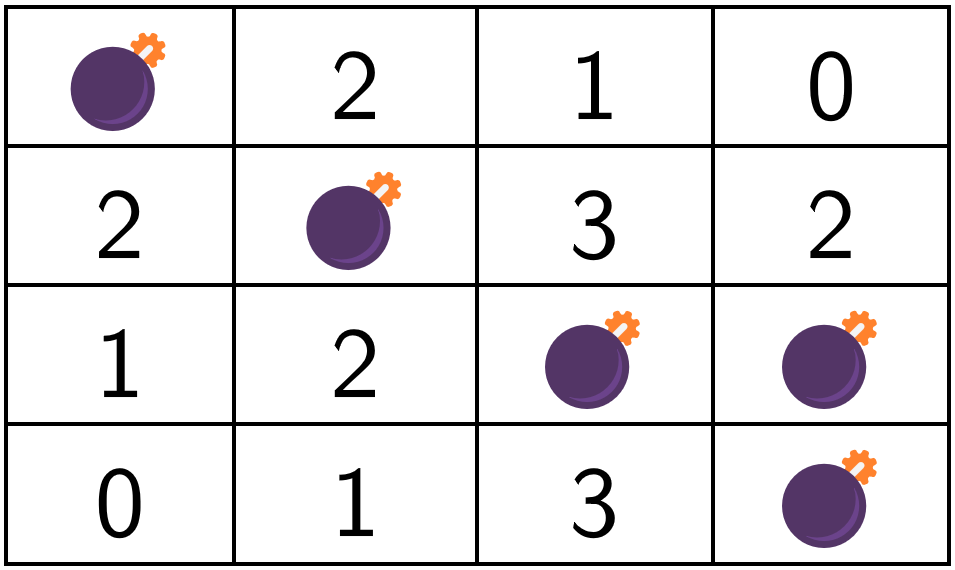
\includegraphics[height = 0.6\textwidth]{Minesweeper/explanation.png}
		\caption{Explanation for all cells}
		\label{fig:minee}
	\end{subfigure}
	\caption{Minesweeper -- Explanation}
\end{figure}
\vspace{-2em}
\textbf{Problem Statement:}\\
Calculate the neighbour count for all cells except at the mines where you have to output the character `M'.% in place of a number.
\begin{testcasesMore}
	{%$t$ \hfill(number of test cases, an integer)\\
	$m\ n$\hfill(space seperated integer pair corresponding to number of rows and columns)\\$k\quad x_1\ y_1\ \quad\cdots\quad x_{k}\ y_{k}$ \hfill($2k+1$ space seperated integers corresponding to number of mines and the $x,y$ co-ordinates of all mines (1-indexed))}
	%These numbers correspond to (number of rows, columns, mines, all co-ordinates of mine (2D, 1-indexed)).}
	{$m\times n$ matrix $A$, where $a_{ij}=\begin{cases}
		\text{`M'}& \text{if there is a mine at $(i,j)$} \\
		\text{number of neighbouring mines of the cell $(i,j)$} & \text{otherwise}
	\end{cases}$}
	{$1 \leq m,n \leq 50$, $1 \leq k \leq m\times n$\\$1 \leq x \leq m$, $1 \leq y \leq n$\\$0 \leq a_{ij} \leq 8$ or $a_{ij}=$ `M'.}%\hfill()
	{4 4\\5\qquad1 1 \quad2 2 \quad3 3\quad3 4\quad4 4}
	{M 2 1 0\\	2 M 3 2 \\	1 2 M M \\	0 1 3 M}
	{https://github.com/paramrathour/CS-101/tree/main/Test Cases/Minesweeper/Input}
	{https://github.com/paramrathour/CS-101/tree/main/Test Cases/Minesweeper/Output}
	{https://github.com/paramrathour/CS-101/tree/main/Starter Codes/Minesweeper.cpp}
\end{testcasesMore}
\begin{note}
	Try implementing the complete minesweeper game :)
\end{note}
\subsection{Gray Code}
A gray code is a rearrangement of binary numbers such that any 2 consecutive numbers differ only in 1 bit.

A simple way to generate n-bit gray code is given below
\begin{itemize}	
	\item Start with an array of $2$ numbers $A = \{0, 1\}$
	\item Repeat the below steps $n-1$ times
	\begin{itemize}
		\item Reverse the array $A$ to get array $A^\prime$  and then append $A^\prime$  to $A$.
		\item Append $0$ to the left of the first half elements of $A$ and\\
		Append $1$ to the left of the second half elements of $A$.
	\end{itemize}
\end{itemize}
\begin{figure}[H]
	\centering
	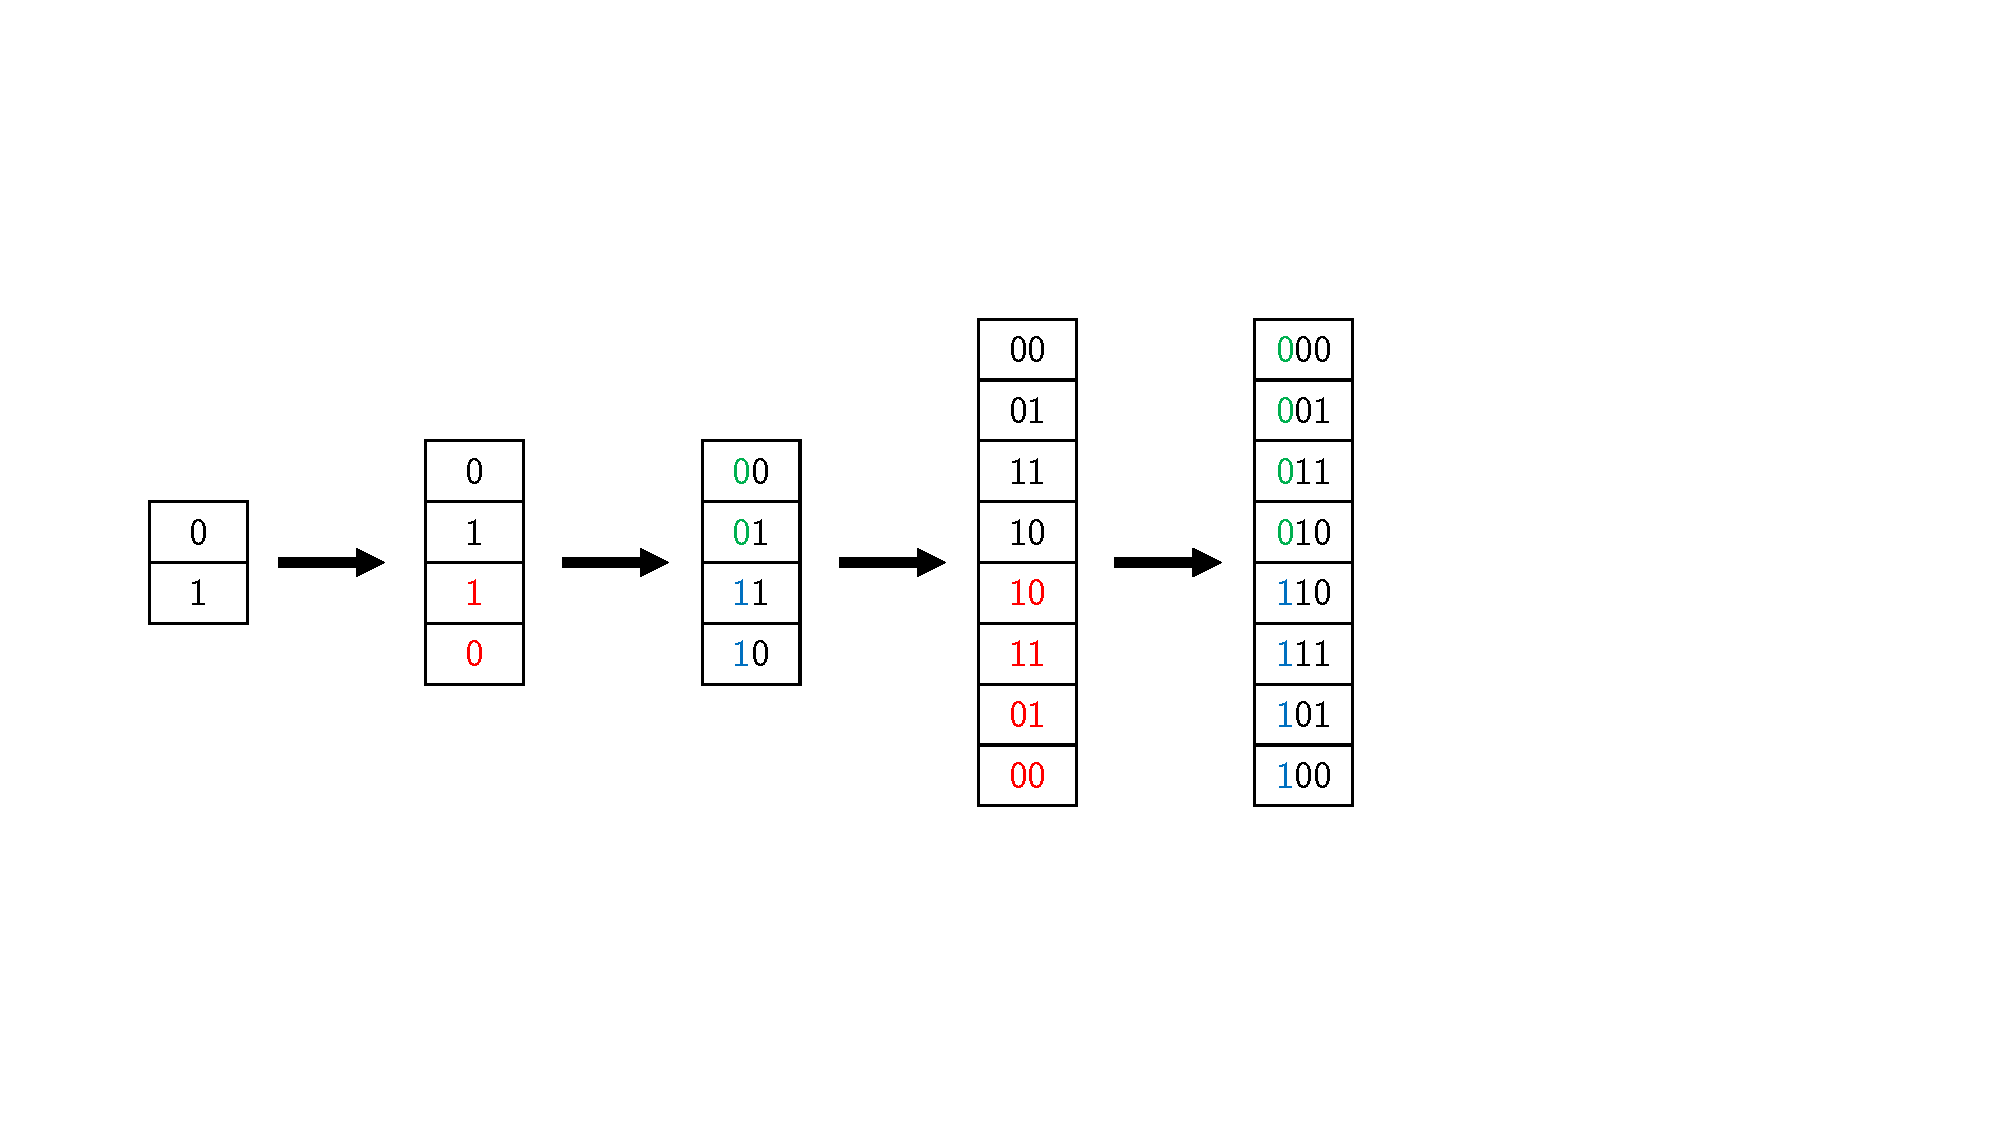
\includegraphics[width = 0.7\linewidth]{Gray Code.pdf}
	\caption{Gray Code -- Generation}
\end{figure}
\vspace{-2em}
\textbf{Problem Statement:}\\
For a given $n$, generate its corresponding Gray Code (i.e. first $2^n$ elements).
\begin{testcasesMore}
	{$n$\hfill(integer)}
	{$2^n$ numbers denoting Gray Code}
	{$1 \leq n \leq 10$}
	{3}
	{000\\001\\011\\010\\110\\111\\101\\100}
	{https://github.com/paramrathour/CS-101/tree/main/Test Cases/Gray Code/Input.txt}
	{https://github.com/paramrathour/CS-101/tree/main/Test Cases/Gray Code/Output.txt}
	{https://github.com/paramrathour/CS-101/tree/main/Starter Codes/Gray Code.cpp}
\end{testcasesMore}